% Figure: the two memory domains exposed by each PE (default heap + GPU heap).
% Referenced in main_spec.tex as fig:mem-domains.
% Regenerate PDF/PNG with:  make -C figures
\documentclass[border=3pt]{standalone}
% Shared preamble for the standalone figure sources in this directory.
% Fonts mirror ../utils/packages.tex so the generated figures match the
% specification's typography. tikz pulls in xcolor automatically.
\usepackage[T1]{fontenc}
\usepackage{mathptmx}
\usepackage[scaled=.90]{helvet}
\usepackage{courier}
\usepackage{tikz}
\usetikzlibrary{positioning,arrows.meta,fit,backgrounds,calc}

\begin{document}
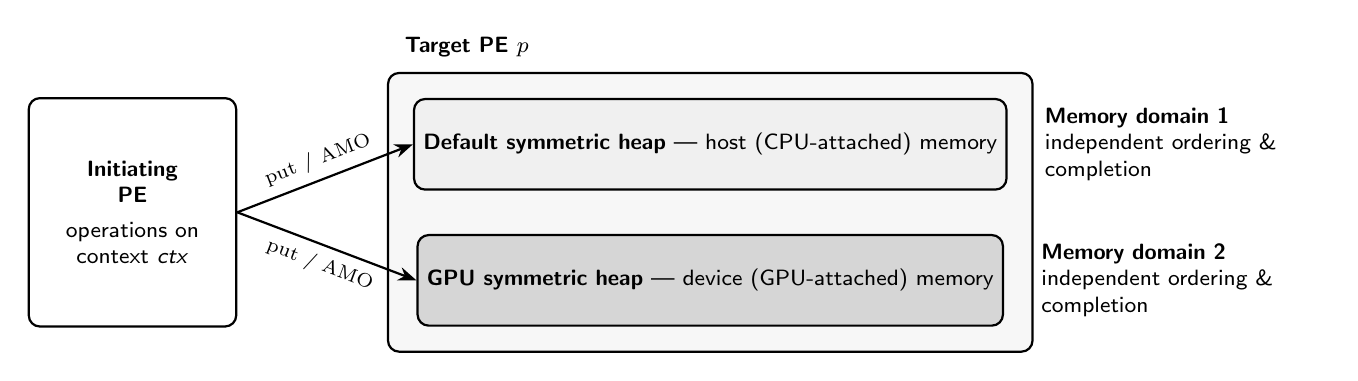
\begin{tikzpicture}[
  font=\footnotesize\sffamily, >=Stealth, node distance=0.55cm and 1.9cm,
  lane/.style={draw, thick, rounded corners, minimum width=6.2cm,
               minimum height=1.15cm, align=center},
]
  \node[lane, fill=black!6] (host)
        {\textbf{Default symmetric heap} --- host (CPU-attached) memory};
  \node[lane, fill=black!16, below=of host] (dev)
        {\textbf{GPU symmetric heap} --- device (GPU-attached) memory};
  \begin{scope}[on background layer]
    \node[draw, thick, rounded corners, fill=black!3, inner sep=9pt,
          fit=(host)(dev)] (pe) {};
  \end{scope}
  \node[font=\footnotesize\sffamily\bfseries, anchor=south west]
        at ([xshift=3pt, yshift=2pt]pe.north west) {Target PE $p$};

  \node[draw, thick, rounded corners, fill=white, align=center,
        text width=2.4cm, minimum height=2.9cm, left=of pe] (src)
        {\textbf{Initiating}\\\textbf{PE}\\[3pt] operations on\\ context \textit{ctx}};

  \draw[->, thick] (src.east) to node[above, font=\scriptsize, sloped] {put / AMO} (host.west);
  \draw[->, thick] (src.east) to node[below, font=\scriptsize, sloped] {put / AMO} (dev.west);

  \node[right=0.35cm of host, text width=3.5cm, align=left]
        {\textbf{Memory domain 1}\\ independent ordering \& completion};
  \node[right=0.35cm of dev, text width=3.5cm, align=left]
        {\textbf{Memory domain 2}\\ independent ordering \& completion};
\end{tikzpicture}
\end{document}
